
% !TEX root = Entwurf_goApp.tex

\section{Entwurfsentscheidungen}
	\subsection{Einleitung}
	Das folgende Dokument beschreibt den Entwurf der goApp und ist nach dem Prinzip top-down aufgebaut.
	Zunächst werden die Entscheidungen bezüglich der Architektur und welche Entwurfsmuster zum Einsatz kommen erläutert.
	Darauf folgen Beschreibungen zu jedem Package und schlussendlich wird auf jede Klasse im einzelnen eingegangen.
	Im Kapitel Sequenzdiagramme werden interne Abläufe graphisch dargestellt und sollen das Zusammenspiel unserer Komponenten verdeutlichen. 
	Im Anhang findet sich ein großformatiges Diagramm mit allen Klassen.
	\subsection{Architektur}
	Die Architektur der goApp ist die Client-Server Architektur. Diese zeichnet sich dadurch aus, dass ein passiver Server Anfragen der aktiven Clients entgegennimmt, bearbeitet und eine Antwort zurück übermittelt. Die Architektur bietet sich in diesem Fall an, da die goApp mehrere Nutzer hat und diese gleichzeitig auf die selben Daten und Services zugreifen können müssen. 
	Ein Client ist in diesem Fall ein Androidgerät und der Server ein auf Linux basierender Webserver.
	Der Entwurf verwirklicht die Client-Server-Architektur dadurch, dass der Client Http-Anfragen an den Server schickt. Der Server stellt den Zugriff auf entsprechende Nutzer, Gruppen und Termin Daten über Servlets zur Verfügung. Diese Daten sind in der Datenbank auf dem Server gespeichert. Diese Daten können über Anfragen des Clients auch geändert werden. Zudem berechnet der Server mithilfe eines Clustering-Algorithmus die Gruppenmittelpunkte, welche dann von den Clients abgefragt werden können.
	 
	3-Schichten?
	
	
	\subsection{Paketstruktur}
	 \includegraphics[width=1.1\textwidth]{Packages.png}

	\subsection{Server \& Client Kommunikation}

	Wir verwenden JavaScript Object Notation Remote Procedure Call (kurz: JSON-RPC) für die Kommunikation zwischen den Clients und dem Server.
	Ein JSON-RPC-Call besteht aus einem JSON-String, der vom Client an den Server geschickt wird, welcher wiederum mit einem JSON-String antwortet
	Durch die Nutzung von JSON-RPC versprechen wir uns eine flexible aber vor allem eine einfache Kommunikation, welche wir genau auf unsere Anforderungen anpassen können.
Durch das explizite angeben der Methode in der Anfrage ist man frei bei der Wahl der Methoden welche ein Servlet zur Verfügung stellt. Bei alternativen wie z.B. REST sind die Methoden eines Servlets gebunden an die Methoden (GET, POST, PUT, Delete...) des HTTP-Protokolls. Dadurch ist man gezwungen seine Methoden dahingehend anzupassen.

	
	\subsection{Server}
	\subsubsection{Modell}
Im Modell werden Benutzer, Gruppen und Events direkt aus der Realität auf die entsprechende Klasse abgebildet. Zusätzlich existieren Klassen die den Standort und Gruppenbeitrittsanfragen der Benutzer darstellen.
Ein Benutzer kann Mitglied in bis zu 20 Gruppen sein, und in jeder Gruppe darf es bis zu 50 Mitglieder geben sowie genau einen Gründer. Bevor ein Benutzer Mitglied einer Gruppe werden kann muss er eine Beitrittsanfrage erstellen.
Pro Benutzer können bis zu 20 Anfragen gleichzeitig existieren. Diese gehören jeweils zu einer Gruppe.
An eine Gruppe können jedoch beliebig viele Anfragen gestellt werden.
Ebenso können in einer Gruppe beliebig viele Events existieren, an denen jeweils alle Gruppenmitglieder teilnehmen können.
Damit die Teilnehmer eines Events sich finden können existiert die Klasse Location, eine Location kann entweder genau einem Benutzer oder genau einem Termin zugeordnet sein. 
Eine genaue Beschreibung aller Klassen des Modells mitsamt ihren Methoden findet sich im Kapitel 3.1.

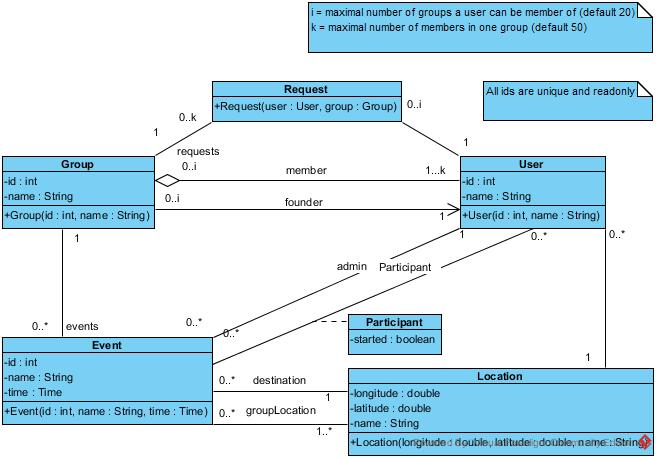
\includegraphics[width=1.1\textwidth]{ModelClassDiagram.jpg}

	\subsubsection{DatabaseManagement}
	Die Klassen des DatabaseManagement sorgen für den Zugriff auf die Datenbank.
	Mittels Hibernate werden die gewünschten Daten aus der Datenbank abgerufen, geändert oder eingefügt und eine entsprechende Meldung an den Aufrufer gegeben.
	Dies ist unsere einzige Schnittstelle zur Datenbank.	
	Eine genaue Beschreibung aller Klassen des DatabaseAdapters mitsamt ihren Methoden findet sich im Kapitel 3.2.

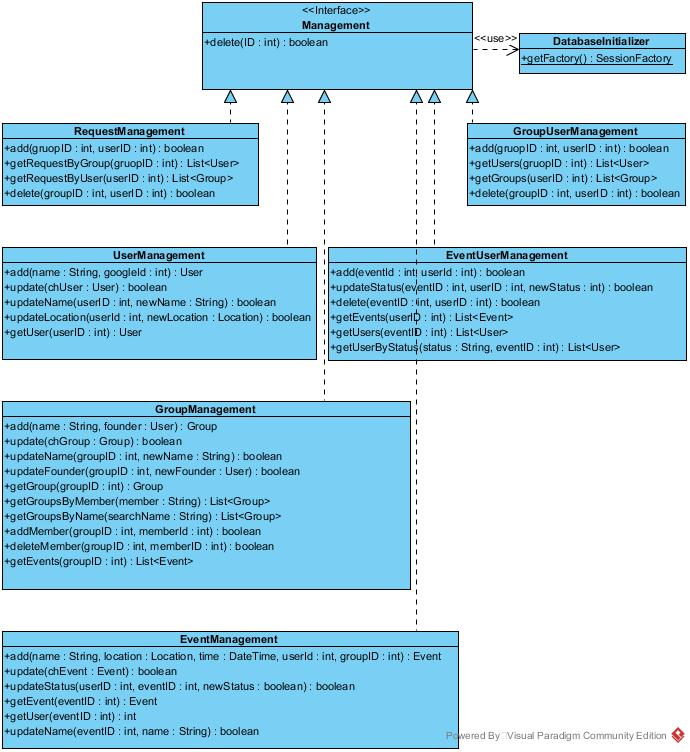
\includegraphics[width=1.1\textwidth]{ManagementClassDiagram.jpg}


	\subsubsection{Hibernate}
	Zur Verwaltung und Erstellung unserer Datenbank wollen wir das Hibernate-Framework nutzen. 
	Dies ermöglicht uns eine objektrelationale Abbildung, sodass wir unsere Java-Objekte in einer relationalen Datenbank speichern können und Beziehungen mit abgebildet werden.
	Ein großer Vorteil ist, dass die Datenbank von Hibernate erstellt und verwaltet wird, sodass spätere Änderungen im Modell einfach umgesetzt werden können.
	Wir nutzen das Hibernate-Framework, in dem wir in unseren Modell-Klassen für alle Klassen und Attribute Java-Annotations setzen.
	
%TODO	\subsubsection{Database}
	%TODO: rausnehmen ??? 	In der Datenbank werden für alle Elemente und Objekte die entsprechenden Daten gespeichert und bei Bedarf ausgelesen. Hierzu wird für jede Klasse des Modells sowie für bestimmte Beziehungen eine Tabelle angelegt.Identifiziert werden die jeweiligen Objekte durch eine eindeutige ID welche bei der Erstellung des Eintrags vergeben wird.Für Benutzer kommt diese ID von Google für die anderen Klassen wird die ID direkt von unserem Server vergeben.TODO: Hier vielleicht noch ein UML-Diagramm erstellen auf dem alle Tabellen sind die wir speichern werden (also auch die Zwischentabellen) und was jeweils gespeichert wird.

	\subsubsection{Clusteringalgorithmus}

Das Clusteralgorithmuspaket gruppiert Standorte und kann den Mittelpunkt mehrerer Standorte berechnen. Wir haben uns dabei dazu entschieden das Entwurfsmuster Strategie zu verwenden, um es zu ermöglichen die Implementierung der Clusteranalyse, sowie der Mittelpunktberechnung abzukapseln und somit für die jeweiligen Bedürfnisse austauschbar zu machen. Einzelne Klassen aus dem Clusteralgorithmuspaket sind aus der Apache Commons Mathematics Bibliothek und müssen somit nicht mehr von uns implementiert werden. Wir verwenden Teile dieser Bibliothek, da sie unter der Apache License steht, gut getestet ist und perfekt zu unserem Projekt passt. Außerdem soll unser Projekt einen Mehrwert generieren und nicht darin bestehen vorhandene Software nachzubauen. Das Clusteralgorithmuspaket kommuniziert direkt mit dem Package database.management und bekommt die Daten nicht von dem Servlet übergeben. Dies hat den Vorteil, dass die benötigten Daten nur von dem Algorithmus abhängig sind, was die Austauschbarkeit unterstützt. Neben den Klassen aus der Apache Bibliothek besteht dieses Paket aus eigenen Algorithmen zur Berechnung des Mittelpunkts bei der Punkte unterschiedlich gewichtet werden, um einen möglichst sinnvollen Mittelpunkt zu erhalten. Da eine wichtige Funktionalität unserer App darin liegt, Standorte der Gruppe auf einer Karte anzeigen zu lassen, legen wir auch einen besonderen Wert auf eine sinnvolle Berechnung der Cluster. Da unsere Erfahrung im Umgang mit Clusteralgorithmen noch nicht sehr groß ist wollen wir noch offen lassen welchen Clusteralgorithmus wir verwenden werden. Wir konnten unsere Auswahl bis jetzt auf den sogenannten DBSCAN-Algorithmus, bzw. den KMEANS-Algorithmus beschränken. Der DBSCAN-Algorithmus ist ein dichtebasierter Clusteralgorithmus und hat gegenüber dem KMEANS-Algorithmus den Vorteil, dass nicht vor der Berechnung klar sein muss wie viele Cluster entstehen sollen. Außerdem arbeitet er mit "Rauschen", bedeutet Punkte die keinem Cluster zugeordnet werden können, werden separat ausgegeben. Dabei arbeitet der Algorithmus mit einem Maximalabstand den Punkte zueinander haben dürfen. 
Der KMEANS-Algorithmus ist einer der am meisten genutzten Algorithmen zur Clusteranalyse und hat im Gegensatz zum DBSCAN-Algorithmus den Vorteil, dass er Cluster unterschiedlicher Dichte erkennen kann. Zudem bietet er ein signifikant besseres Laufzeitverhalten. Das Problem, dass in unserem Fall die Zahl der Cluster vor der Berechnung noch nicht feststeht, kann durch Evaluationsalgorithmen gelöst werden. Die Evaluationsalgorithmen werden in der Apache Bibliothek erst ab Version 4.0 angeboten, welche noch nicht offiziell veröffentlicht wurde, deren Clusterbibliothek jedoch schon gut getestet online verfügbar ist.
Wir werden in der Implementierungsphase entscheiden ob wir die Apache Commons Math Bibliothek 4.0 oder 3.6.1 verwenden, da doch ein enormer Mehrwert durch die Version 4.0 entsteht.
  \newline
	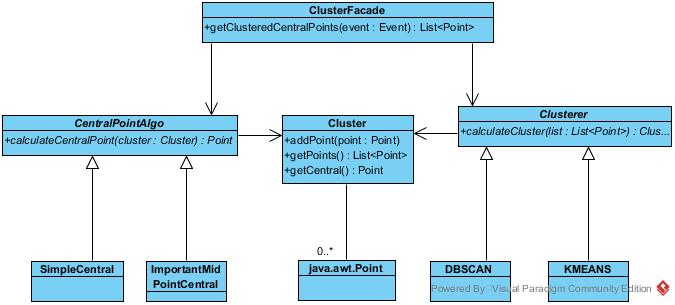
\includegraphics[width=1.1\textwidth]{AlgorithmClassDiagram.jpg}

	\subsubsection{Servlets}

	Die Servlets nehmen die Anfragen der Clienten entgegen. Diese ist immer ein JSON-String welcher von den Servlets ausgelesen und danach entsprechend behandelt wird. Die Servlets leiten die erhaltenden Anfragen entweder an die Datenbankverwaltung oder an den Algorithmus weiter und schicken das Ergebnis an den Clienten.
Die Servlets fungieren so als Schnittstelle zwischen den Anfragen des Clients und der eigentlichen Arbeit die auf dem Server vollbracht wird. 
Die Servlets sind in ihren Aufgabenbereichen unabhängig voneinander und auf das Modelll angepasst, so gibt es z.B. ein Servlet was alle Anfragen bezüglich eines Events beantwortet und ein weiteres welches sich um die Handhabung der Gruppenbeitrittsanfragen kümmert.
Die Servlets sind auf die Services des Clients zugeschnitten, ein Servlet beantwortet also nur Anfragen von genau einem Service.
Für eine weitere Funktionalität kann also einfach ein neuer Service mit einem neuem Servlet unabhängig von allen anderen erstellt werden was den Entwurf erweiterbar macht.   

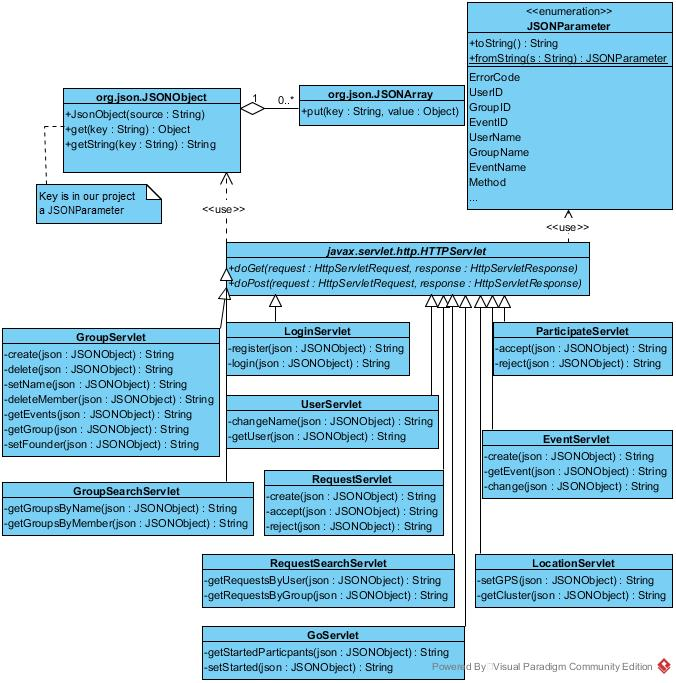
\includegraphics[width=1.1\textwidth]{ServletsClassDiagram.jpg}


	\subsection{Client}
%TODO
	Der Client implementiert das Entwurfsmuster Model-View-Controller was unseren Entwurf flexibel und austauschbar macht.
	\subsubsection{Services}
	Die Services sind der Controller des Clients und damit für die Steuerung zuständig. Hauptaufgabe ist es die Kommunikation zwischen der View und dem Server zu gewährleisten, aber auch Hintergrundprozesse anderer Art, wie das erstellen eines Timers, gehören in ihren Aufgabenbereich.
Sie sind, wie die Servlets, so entworfen, dass jeder Service seinen eigenen Aufgabenbereich übernimmt.
Von unserer App werden folgende Services implementiert:
\newline
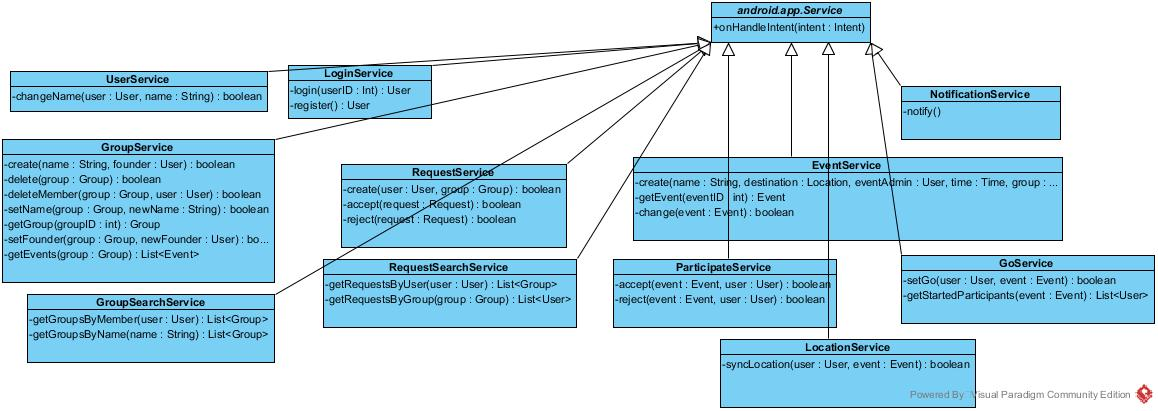
\includegraphics[width=1.1\textwidth]{Controler.jpg}

	\subsubsection{Activities}
	Alle Activities setzten sich aus XML-Dateien zusammen und bilden gemeinsam die View des Users.
Sie nehmen als erstes Benutzerinteraktionen entgegen, leiten diese an den entsprechenden Service weiter und geben dem User entsprechendes Feedback.
	\newline
	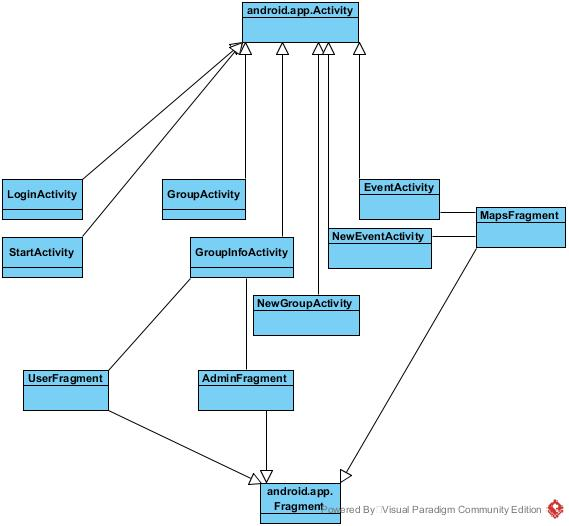
\includegraphics[width=1.1\textwidth]{ViewClassDiagram.jpg}
	
	\subsubsection{Modell}
Das Modell versucht die Realität auf die Daten des Servers und der Applikation abzubilden und ist von dem Controller und der View unabhängig. 
%TODO Entwurfsmuster ?
Das Modell auf dem Client entspricht dem Modell des Servers.

	\subsubsection{ServerConnection}
	Die Klasse HTTPConnection bildet die Schnittstelle zwischen dem Server und dem Client. Die Services schicken Anfragen an sie. Diese werden über eine HTTP-Verbindung an die entsprechenden Servlets des Servers weitergeleitet und deren Antwort gibt HTTPConnection wieder an den Service zurück.
		\newline
		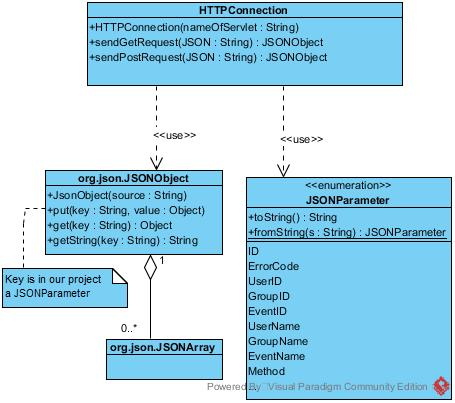
\includegraphics[width=1\textwidth]{HTTPClientClassDiagram.jpg}

	\subsection{Fehlerbehandlung}
Wenn auf dem Server ein Fehler auftritt wird dieser vom Servlet abgefangen und in dem JSON-String der Antwort eingetragen. Dafür gibt es extra ein Errorcode Parameter in der Klasse JSONParameter. Durch diesen Fehlercode in der Serverantwort wird dem Client der Fehler mitgeteilt.\par

Da auf dem Client keine wichtigen Daten gespeichert sind werden hier die auftretenden Fehler nur an den Benutzer mit einer aussagekräftigen Meldung weiter gegeben. Außerdem werden alle Informationen atomar übergeben und können zusätzlich noch neu vom Server geladen bzw. an den Server geschickt werden. \par

Unsere Kommunikation beinhaltet keine sensiblen Daten, die explizit nur einmal gesendet werden sollen. Dadurch werden keine zustandsichernden Maßnahmen benötigt, um auf den Zustand vor dem Fehler zurückkehren zu können und z.B. gescheiterte Anfragen neu zu stellen.
	



		


	\newpage
